\section{Metody interpolacyjne}
\subsection{Regula falsi}
\begin{frame}{Metody interpolacyjne - Regula falsi}
	\centering   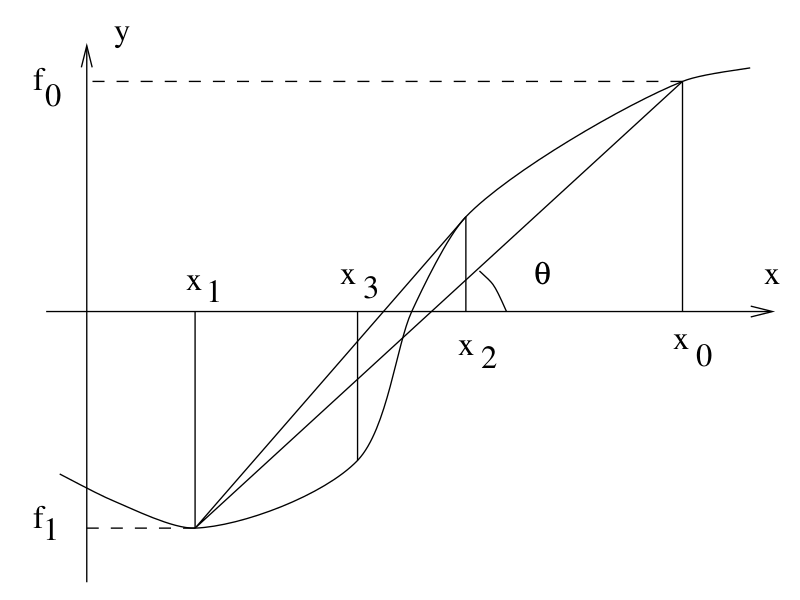
\includegraphics[width=.7\linewidth]{img/7/7_6_1}
\end{frame}
%%%%%%%%%%%%%%
\begin{frame}{Regula falsi}
	\begin{enumerate}
		\item $x_{0}$, $x_{1}$ : $f(x_{0}) \cdot f(x_{1}) < 0$
		
		\item linia prosta: $\frac{f_{0} - f_{1}}{x_{0} - x_{1}} = \frac{f_{0}}{x_{0} - x_{2}} \Rightarrow x_{2} = \frac{f_{1}}{f_{1} - f_{0}} x_{0} + \frac{f_{0}}{f_{0} - f_{1}}x_{1}$
		
		\item sprawdzenie 	$\left. \begin{array}{ll}
								f_{1} \cdot f_{2} < 0\\
								f_{0} \cdot f_{2} < 0
							\end{array}\right\} \Rightarrow x_{3} \ldots$\\
	\end{enumerate}
	- wolno zbieżna do poj. pierwiastka (zbieżność liniowa) \quad $\clubsuit ZAD$
\end{frame}
%%%%%%%%%%%%%%
\begin{frame}{Regula falsi}
	Wyjątkowo trudny przypadek:\linebreak
	\begin{center}
		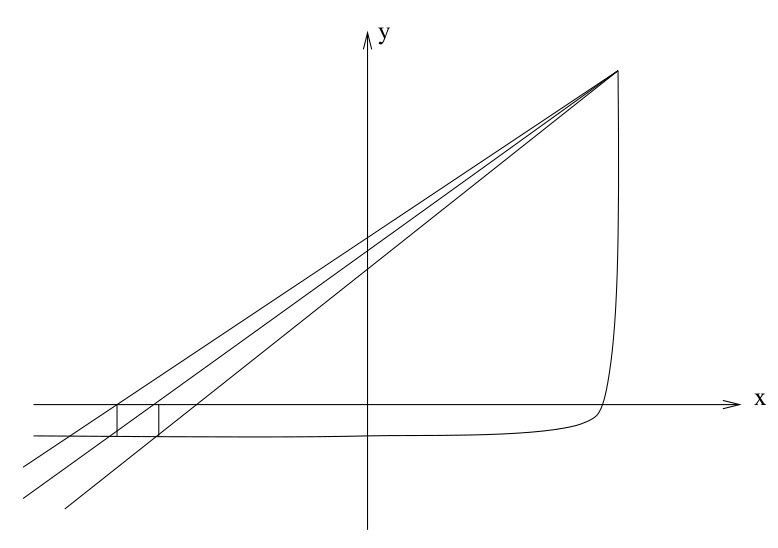
\includegraphics[width=.65\linewidth]{img/7/7_6_2}
	\end{center}
	ważne dla RF: wszystkie iteracje po tej samej stronie pierwiastka
\end{frame}
%%%%%%%%%%%%%%
\subsection{Metody Illinois i Pegasus - ulepszenie RF}
\begin{frame}{Metody Illinois i Pegasus - ulepszenie RF}
	\begin{enumerate}
		\item $x_{i}$, $x_{i+1}$, $x_{i+2}$: $\begin{cases}
			f_{i} \cdot f_{i+1} \qquad <0 $ $ \leftarrow $ obejmują pierwiastek$\\
			f_{i+1} \cdot f_{i+2} \quad <0
		\end{cases}$
		
		\item stosujemy RF do $x_{i}$, $x_{i+2}$ $\Rightarrow$ $x_{i+3}$ ale z: $f_{i} = f_{i}^{*} = \alpha \cdot f_{i}$
		
		\item gdy $f_{i+2} \cdot f_{i+3}$ $\begin{cases}
			< 0 $ - RF dla $ x_{i+2}$, $ x_{i+3}\\
			> 0 $ - zmodyf. RF dla $ x_{i}$, $x_{i+3}
		\end{cases}$
	\end{enumerate}
\end{frame}
%%%%%%%%%%%%%%
\begin{frame}{Metody Illinois i Pegasus - ulepszenie RF}
	\centering 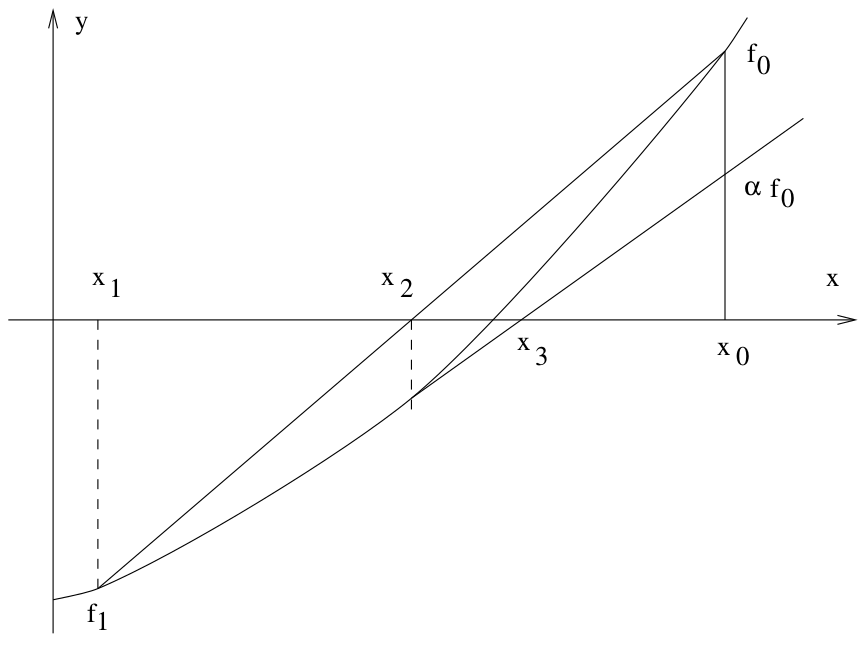
\includegraphics[width=.7\linewidth]{img/7/7_6_3} \linebreak
	\textbf{Illinois} $\rightarrow$ $\alpha = \frac{1}{2}$, \quad \textbf{Pegasus} $\rightarrow$ $\alpha = \frac{f_{0}}{f_{1} + f_{0}}$
\end{frame}
%%%%%%%%%%%%%%
\subsection{Metoda siecznych}
\begin{frame}{Metoda siecznych}
	\centering 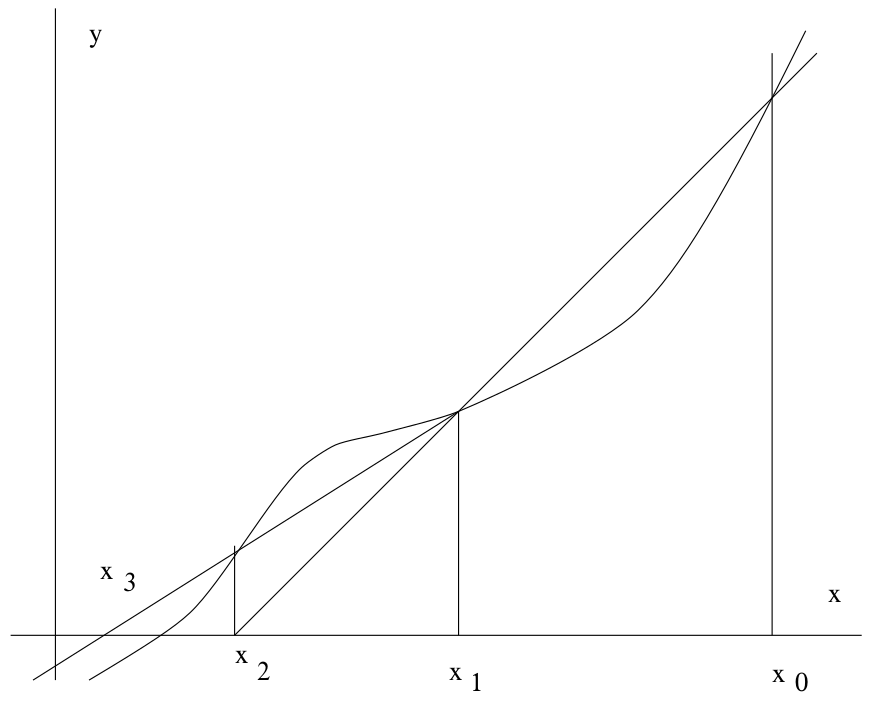
\includegraphics[width=.8\linewidth]{img/7/7_6_4}
\end{frame}
%%%%%%%%%%%%%%
\begin{frame}{Metoda siecznych}
	- $(x_{0}, x_{1})$\linebreak
	- $f_{0} \cdot f_{1}$ - nie badamy\linebreak
	linie prosta $(x_{0}, f_{0})$, $(x_{1}, f_{1})$ $\ldots$
	\[
		x_{i+2} = x_{i+1} - \underbrace{\frac{x_{i+1} - x_{i}}{f_{i+1} - f_{i}}}_{(*)} \cdot f_{i+1}
	\]
	$(*)$ - jak N-R z takim przybl. $f'(x_{i})$ \linebreak\linebreak
	- rząd zbieżności $\sim$ 1.62 \hspace{5cm} $\clubsuit ZAD$\linebreak
	- lepsza od RF\linebreak
	- gorsza od NR - lecz bez $f'$ !
\end{frame}